%%%%%%%%%%%%%%%%%%%%%%%%%%%%%%%%%%%%%%%%%%%%%%
%%%%% Default format: 12pt single column %%%%%
%% 12pt is the minimum font size allowed !! %%
%% This applies to everything, including    %%
%% references, figure captions, and tables  %%
%% ==> Proposals not compliant to this will %%
%%     be rejected. See Section 5.3.1 in    %%
%%     the ALMA Proposer's Guide            %%
%%%%%%%%%%%%%%%%%%%%%%%%%%%%%%%%%%%%%%%%%%%%%%

\documentclass[12pt,a4paper]{article}  %% DO NOT CHANGE to 11pt or less !

\usepackage[numbers]{natbib}
\usepackage{hyperref}
\usepackage{graphics,graphicx}
\usepackage{xspace}
\usepackage{amsmath,amssymb}
\newcommand{\msun}{\ensuremath{\mathrm{M}_\odot}\xspace}
\newcommand{\kms}{\ensuremath{\mathrm{km~s}^{-1}}\xspace}
\newcommand{\percc}{\ensuremath{\mathrm{cm}^{-3}}\xspace}
\newcommand{\persc}{\ensuremath{\mathrm{cm}^{-2}}\xspace}

\newcommand{\mnras}{MNRAS}
\newcommand{\apj}{ApJ}
\newcommand{\jcp}{JCP}
\newcommand{\aap}{A\&A}

\usepackage[table]{xcolor}% http://ctan.org/pkg/xcolor


\usepackage{titlesec}
\titlespacing{\section}{12pt}{6pt}{8pt}
\titlespacing{\subsection}{12pt}{6pt}{8pt}

\newlength\tindent
\setlength{\tindent}{\parindent}
%\setlength{\parindent}{0pt}
\renewcommand{\indent}{\hspace*{\tindent}}


\usepackage{tcolorbox}
\usepackage{paralist}

\renewenvironment{thebibliography}[1]{%
  %\section*{\refname}%
  \textsc{\textbf{References:}}
  \let\par\relax\let\newblock\relax%
  \inparaitem[{[}1{]}]}{\endinparaitem}
  
\usepackage{etoolbox}
\makeatletter
\patchcmd{\@lbibitem}{\item[\hfil\NAT@anchor{#2}{\NAT@num}]}{\item[\NAT@anchor{#2}{\NAT@num}]}{}{}
\makeatother



%%%%%%%%%%%%%%%%%%%%%%%%%%%%
%%%%%% Page dimensions %%%%%
%%%%%%  DO NOT CHANGE  %%%%%
%%%%%%%%%%%%%%%%%%%%%%%%%%%%

\textheight=247mm
\textwidth=180mm
\topmargin=-7mm
\oddsidemargin=-10mm
\evensidemargin=-10mm
\parindent 10pt

%%%%%%%%%%%%%%%%%%%%%%%%%%%%%
%%%%% Start of document %%%%% 
%%%%%%%%%%%%%%%%%%%%%%%%%%%%%

\begin{document}
\pagestyle{plain}
\pagenumbering{arabic}
\newcommand{\arcsec}{"}


 
% The title, abstract and list of investigators should NOT be included in the
% Scientific justification. The title and abstract are put automatically on the cover page.

%%%%%%%%%%%%%%%%%%%%%%%%%%%%%%%%%%%%%%%%%
%%%%% Body of science justification %%%%%
%%%%%%%%%%%%%%%%%%%%%%%%%%%%%%%%%%%%%%%%%

%% ENTER TEXT, FIGURES AND TABLES BELOW
%% Minimum font size for all text, references, figure captions, and tables is 12pt
%% Proposals not compliant to this will be rejected. See Section 5.3.1 in the ALMA Proposer's Guide.


\vspace{-0.5em}
\begin{center}
\large
\textbf{{Scientific Justification: \emph{The MUBLO is a unique source}}}
\end{center} 
\vspace{-0.5em}


% ALMA uses two systems to review the proposals submitted in the Main Call.
% All proposals requesting less than 50 h on the 12-m Array and all ACA stand-alone proposals
% requesting less than 150 h on the 7-m Array will be reviewed by Distributed peer review
% (see Sections 5.7.1 and 1.2.2 of the Proposer's Guide).
% All Large Programs will be reviewed by Panels. 
% Additionally, both systems will follow a dual-anonymous procedure, in which the proposers
% do not know who are the reviewers and the reviews do not who are the proposers.
%
% Please refer to the guidelines before writing your proposal:
%     https://almascience.org/proposing/alma-proposal-review/dual-anonymous
%
% In the following part, describe the scientific background of the project,
% pertinent references and previous work relevant to this 
% proposal, together with any figures and tables that you judge necessary
% (use the following two examples as templates, or remove)
% Please do not disclose the name(s) of the proposer(s), and write the proposal in a way
% such that the proposer(s) cannot be identified. 
 
%-----------------------------Figure Start---------------------------

% The 'scale' parameter below allows you to scale the figure so that it fits within the page.
% In this case the figure was scaled to 20% of its original size.
% Note: for .png files one has to use pdflatex, not classic latex
%
% Minimum font size for references: 12pt 
% Proposals not compliant to this will be rejected. See Section 5.3.1 in the ALMA Proposer's Guide.
A compact (barely resolved at 1\arcsec~ resolution) millimeter source with extremely broad line width has recently been detected in the Galactic Center \citep{Ginsburg2024}.
This source, G0.02467-0.0727, called the Millimeter Ultra-Broadline Object (MUBLO) by those authors, is detected both in continuum and in very broad line emission (FWHM $\sim165~\kms$; Fig. \ref{fig:coarse_spectra}) in emission lines of CS and SO.
It is not detected at any other wavelength from X-ray to radio.
Many hypotheses for the nature of this source have been evaluated, and it was found that none are presently satisfactory (see Table \ref{tab:hypotheses}).
The MUBLO is an exciting mystery that, at least for now, can only be further investigated by ALMA.

\begin{tcolorbox}
\noindent 
We propose observations to measure the gas conditions in the MUBLO and determine what conditions drive its unique chemistry.
\end{tcolorbox}

\begin{figure}[htp!]
    \centering
    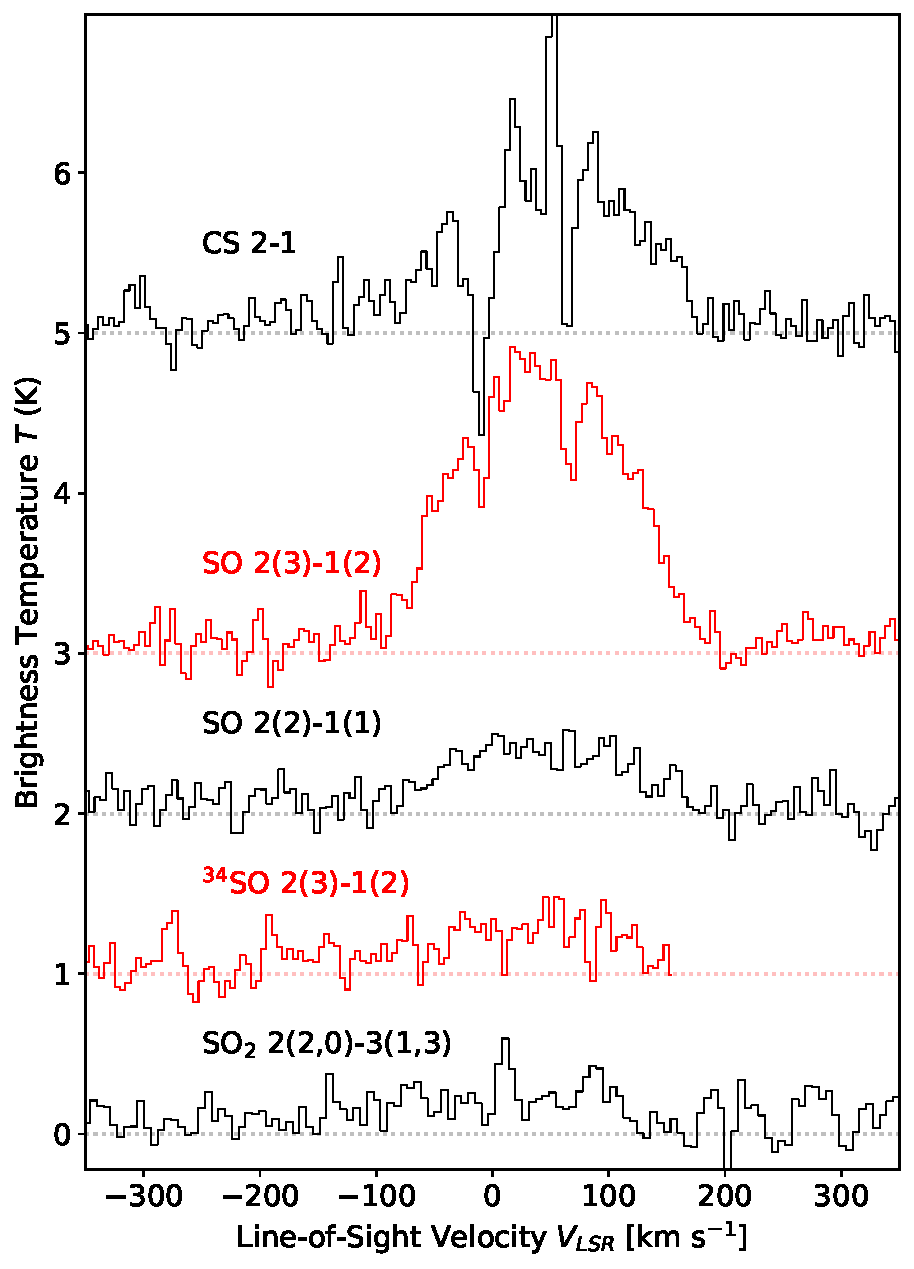
\includegraphics[width=0.36\textwidth]{figures/CSandSO_Overlays.pdf}
    %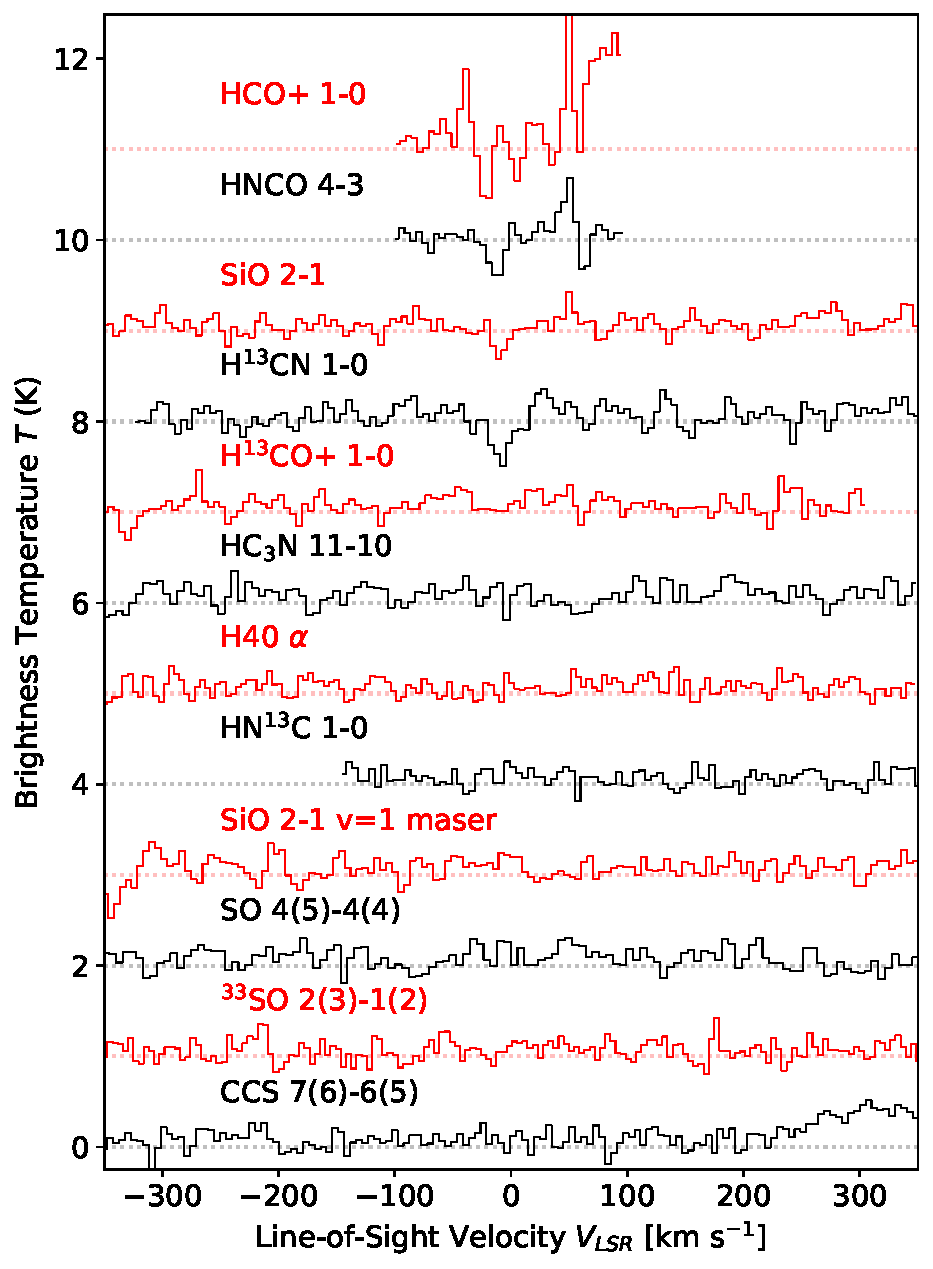
\includegraphics[width=0.49\textwidth]{figures/NonDetection_Overlays.pdf}
    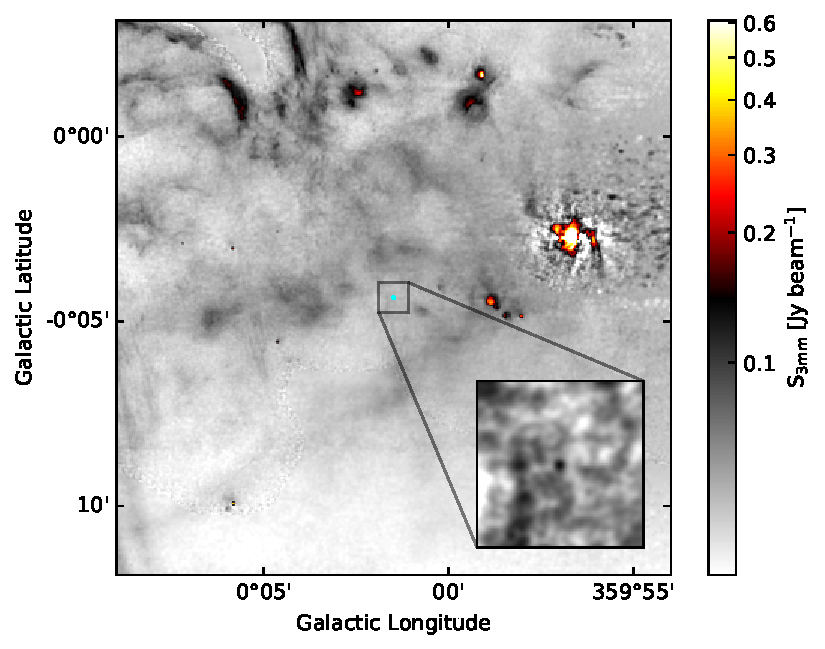
\includegraphics[width=0.63\textwidth]{figures/MUSTANG3mmContext.pdf}
    \caption{(left) Spectra of detected lines in ALMA archival spectral coverage.
    Only CS, SO, and SO$_2$ are detected. (right) Continuum image showing the MUBLO in spatial context. Sgr A* is on the right side of the zoomed-out image.
    %Figure \ref{fig:coarse_spectra_withTP} shows the same data with the Total Power spectra, which covers larger physical scales ($\sim2$ pc), overlaid.
    }
    \label{fig:coarse_spectra}
\end{figure}

\textbf{Source property summary:}
The continuum emission has a spectral index $\alpha\approx3.3$, suggesting that it is from dust.
It is detected in all three ALMA observations that overlap on the sky (two 12M data sets in B3, one 7M in B7) and an SMA DDT observation in B6 (priv. comm.).
The line emission is detected in several transitions of CS and SO isotopologues and exhibits a line width FWHM $\approx165$ \kms (Fig. \ref{fig:coarse_spectra}).  The line profile appears Gaussian.
The emission is weakly spatially resolved in existing 2" resolution data, coming from an area on the sky $\lesssim1"$ in diameter ($\lesssim10^4$ AU at the distance of the GC).
The centroid velocity is $v_{LSR}\approx40-50$ \kms, which suggests the object is genuinely in the Galactic Center and is possibly associated with the 50 \kms cloud.
There is a tentative detection (10$\sigma$ accounting for statistical error only; the systematic errors are difficult to quantify) of a velocity gradient of 11000 \kms pc$^{-1}$.
Two independent SO lines are detected, and assuming LTE conditions, the gas temperature is $T_\mathrm{rot}\approx 14$ K, much colder than seen in typical Galactic Center clouds (Fig. \ref{fig:LTErotationdiagram}).
However, with the limited set of lines presently detected, it is also possible that the emission is coming from low-density, subthermally excited gas.
Despite the high velocity dispersion, no emission is observed from SiO in the observed SiO 2-1 transition, suggesting that there are no strong ($\gtrsim10~\kms$) shocks in the molecular gas.
There are no detections at other wavelengths, including X-ray with Chandra, XMM-Newton, and NUSTAR, infrared with HST and Spitzer, and radio with VLA and MEERKAT.


\textbf{What is it?}
Several explanations were considered for this source, including protostellar outflow, explosive outflow, collapsing cloud, evolved star, stellar collision, high-velocity cloud, intermediate mass black hole, and background galaxy (Table \ref{tab:hypotheses} \citep{Ginsburg2024}).
Most of these conceptual models are inconsistent with the data in at least one way, but the data are not presently very constraining.
In this proposal, we will image the source in the continuum at high resolution to verify the dusty nature of the source and map its internal structure.
With the higher resolution observations of the previously detected lines, we will  determine whether the possible velocity gradient is real and resolve the kinematic structure structure to determine whether it's an outflow, a disk, or something else entirely.

The most exciting possibilities for this source are that it is an intermediate mass black hole (IMBH), it is a very massive, very obscured isolated young stellar object (YSO), or it is a stellar merger remnant.
But none of these models can explain the unique chemistry observed so far:
The MUBLO is rich in CS and SO, but exhibits no emission in common hydrogenic molecules (HCN, HCO$^+$, HC$_3$N, HNCO) or, despite the very broad line width, in SiO.
The deficiency in these molecules makes the MUBLO totally unlike any known stellar merger remnants, evolved stars, or YSOs.
While the observed chemistry can be explained with PDR and CRDR models \citep{Ginsburg2024}, it is difficult to reconcile the observed chemistry with the observed high velocity dispersion, which under most circumstances would imply that strong shocks, producing SiO and HNCO, should be dominant.


\begin{table}[htp]
    \centering
    \begin{tabular}{|c|c|c|c|c|c|c|c|}
         \hline
         Hypothesis & Broad & No IR & No X-ray & Gaussian & $X_{SO}$, $X_{CS}$ & No SiO & Size \\
         \hline
         IMBH \cellcolor{yellow!25} & \cellcolor{green!25}+ & \cellcolor{green!25}+ & \cellcolor{red!25}- & \cellcolor{red!25}- & & & \cellcolor{green!25}+\\
         \hline
         Stellar Merger \cellcolor{yellow!25} & \cellcolor{green!25}+ & \cellcolor{red!25}- & & & \cellcolor{green!25}+ & \cellcolor{red!25}-  & \cellcolor{green!25}+\\
         \hline
         YSO  \cellcolor{yellow!25} & \cellcolor{red!25}- &  \cellcolor{green!25}+ & & \cellcolor{green!25}+ & \cellcolor{red!25}- & \cellcolor{red!25}- &\cellcolor{green!25}+  \\
         \hline
         Protostellar Outflow \cellcolor{orange!25} & \cellcolor{green!25}+ & \cellcolor{red!25}- & & \cellcolor{red!25}- & \cellcolor{red!25}- & \cellcolor{red!25}-  & \cellcolor{red!25}-\\
         \hline
         Supernova \cellcolor{orange!25}& \cellcolor{green!25}+ & \cellcolor{green!25}+ & \cellcolor{red!25}- & & \cellcolor{red!25}- & \cellcolor{red!25}- & \\
         \hline
         (pre)Planetary Nebula \cellcolor{orange!25}& \cellcolor{red!25}- & \cellcolor{red!25}- & &  \cellcolor{green!25}+ & \cellcolor{green!25}+ & \cellcolor{red!25}- & \\
         \hline
         Background Galaxy \cellcolor{red!25}& \cellcolor{green!25}+ & \cellcolor{red!25}- & & & \cellcolor{red!25}- &  & \cellcolor{red!25}-\\
         \hline
         High-velocity Compact Cloud  \cellcolor{red!25}& \cellcolor{green!25}+ & \cellcolor{green!25}+ & \cellcolor{green!25}+ & \cellcolor{red!25}- & \cellcolor{red!25}- & \cellcolor{red!25}- & \cellcolor{red!25}-\\
         \hline
    \end{tabular}
    \caption{Hypotheses that have been evaluated and the evidence for (green +) and against (red -) them; blank means the evidence is neither for nor against.
    The overall weight given to the hypothesis is given by its color code - yellow are not entirely ruled out, orange are strongly disfavored but still possible, and red are very low likelihood.
    There is at least one strong item of evidence against each hypothesis considered.
    }
    \label{tab:hypotheses}
\end{table}



\begin{figure}
    \centering
    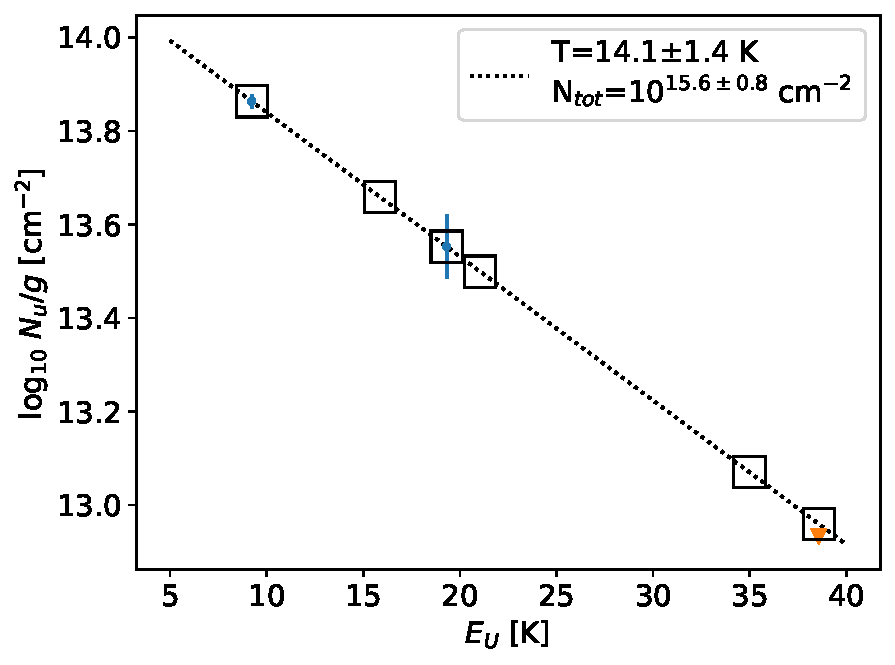
\includegraphics[width=0.49\textwidth]{figures/LTE_rotationdiagram_fit_plannedobs.pdf}
    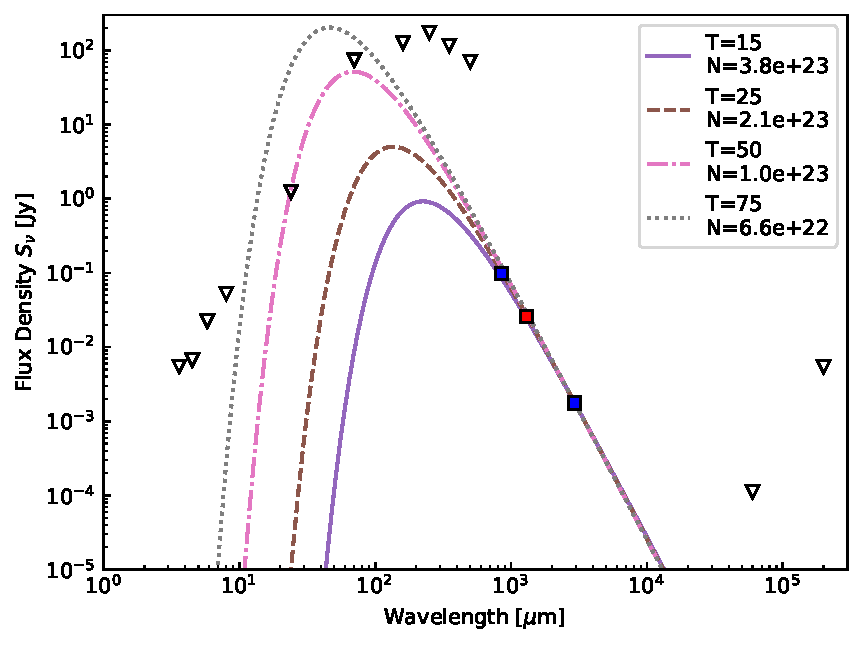
\includegraphics[width=0.49\textwidth]{figures/SED_with_upperlimits_VLA_SMA.pdf}
    \caption{(left) Rotation diagram showing the best fit for the SO lines.
    With only two measured lines (blue), we cannot tell whether the lines are in LTE and genuinely cold or are instead sub-thermally excited.
    We propose here to observe several additional lines, marked in black squares.
    (right) Continuum spectral energy distribution. Except for the ALMA (850 $\mu$m and 3mm; blue) and SMA (1.3mm; red) data points, all are upper limits.  The modified blackbody curves show that the dust temperature is limited to be $T_D<50$ K.
    }
    \label{fig:LTErotationdiagram}
\end{figure}


\vspace{-0.5em}
\begin{center}
\large
\textbf{{Observations \& Analysis Plan:\\ \emph{Measure resolved excitation conditions and search for lines}}}
\end{center} 
\vspace{-0.5em}
Our main science objective is to measure the excitation conditions in the molecular gas by observing many lines of SO and CS, the only species so far detected.
We select bands covering CS 2-1, 3-2, 5-4, and 7-6.
These bands cover multiple transitions of SO.

The first key aim is to determine whether the gas (and dust) temperature is really as cold as implied by the two-line rotation diagram shown in Figure \ref{fig:LTErotationdiagram}.
Then, independent of the temperature, we will use deviations from LTE excitation to determine the (resolved) gas density.
The need to measure the density, which is a key parameter in chemical models, drives the need for lines spanning a wide range of frequencies.
Multi-level line observations of CS and SO, interpreted with both LTE population diagrams and non-LTE radiative transfer models, constrain the origin and physical conditions of the CS and SO emitting gas in the MUBLO (Figure \ref{fig:csradex}).


%Fig. \ref{fig:LTErotationdiagram} shows that the dust is cold enough that the B9 data strongly differentiate different temperature models).

The second key goal is to find what other molecules exist in the MUBLO.
While so far no other molecular species have been detected, it is unlikely that only CS and SO molecules are present.
Chemical models (Meudon \& UCLCHEM) predict that OCS should be highly abundant and potentially even brighter than SO.
%We therefore observe OCS ...
%With both CS and SO detected, it is quite likely that CO is present and abundant; however, CO is also abundant everywhere along this very busy line-of-sight, so higher excitation CO lines (CO 3-2) and rarer isotopologues ($^{13}$CO, C$^{18}$O) are needed to measure the CO abundance
We target several classes of molecules:
\begin{itemize}
 \item SO, SO$_2$ and CS, because they have been detected already and their line ratios can be used to measure the temperature and density \citep{Ginsburg2024}.
 \item Other sulfur-bearing dense gas tracers, including H$_2$CS and OCS.  Given that sulfur-bearing molecules are the only ones so far detected, these are promising next molecules to identify.
 \item Shock tracers (SiO and SiS) at different frequencies to verify the lack of shock-tracing silicon molecules and strengthen their limits.
 \item H$_2$S, SH$^+$, HCS$^+$, and C$_3$H$^+$ to search for the photon-dominated region (PDR) that denotes the edge of the object \citep{Pety2012,McGuire2014}.
       As a dense, molecular object embedded in a harsh, UV-rich radiation field ($G_0\sim10^3-10^4$), there should be a PDR edge.%, which is efficiently traced by C$_3$H$^+$
 \end{itemize}


% \begin{enumerate}
%     \item Resolved observations of the structure of the molecular feature.  We should aim for resolution $10\times$ better than currently achieved, which is straightforward with ALMA and can be requested at several wavelengths in the upcoming Configuration 6 in June 2024.  This is the key measurement, since the shape of the kinematic structure should be different for all of the above hypotheses (e.g., a circumstellar disk will have a Keplerian curve, while a galactic inner disk would likely be either solid-body or flat).  
%     \item A better molecular inventory.  Observations of HCN, HCO+, HNCO would be nice.  CO isotopologues, including very rare ones (C$^{17}$O, $^{13}$C$^{18}$O) should be included to avoid CMZ optical depth problems.  We should brainstorm other important species.  For example, H$_2$CS and H$_2$CO may be useful for better constraining the sulfur chemistry and the gas temperature.
%     \item A better physical characterization.  Additional transitions of CS and SO are necessary to measure the excitation.  Is the temperature really as low as we measure, or is the density low and we are instead seeing non-LTE conditions?
% \end{enumerate}

Our sensitivity goal is to detect SO lines in all bands so we can measure the gas temperature and density.
We set our sensitivity target to 0.25 K in 5 \kms channels for the higher frequency bands and somewhat worse for the low frequencies.
The detected lines have peak brightness $T_B\sim2$ K over a 2" beam, which would be $\sim200$ K in the proposed 0.2" beam if the emission remains unresolved; we expect the real brightness to be somewhere between these values (Figure \ref{fig:csradex}).
%The lower frequency and excitation lines are expected to be closer to optically thick when resolved

Our resolution target is set to 0.2" ($\sim1600$ AU), which is 10$\times$ better (linearly) than the observations in which the MUBLO was first detected.
This moderately high angular resolution is critical for testing the hypotheses in Table \ref{tab:hypotheses}:
for every one of these hypotheses, the emission is expected to be structured such that it is brighter on smaller scales.
If the MUBLO's line width is produced by a disk of any kind, it must be at least somewhat inclined to the line of sight.
Several models (merger, YSO) should be centrally heated and therefore centrally peaked in line excitation and brightness, while others (IMBH, explosion) may be brighter further out and dominated by shocks.
However, since most of those models were ruled out by the original data, we simply need high resolution to help us generate new hypotheses and figure out what it actually is.
The selected resolution is the ideal compromise between high resolution and brightness sensitivity and can be achieved at all selected ALMA bands, enabling a fair band-to-band comparison.

We show a set of non-LTE RADEX models of CS in Figure \ref{fig:csradex} to demonstrate that, if the gas is at moderate density ($n<10^8$ \percc), we will be able to measure the density using CS line measurements in the lower bands (B3, B4) and upper limits at the high end (B6, B7).
The model shown is a reasonable prediction of what we might see, since we adapt the 2" resolution for the higher resolution by assuming a filling factor 0.1 (it is constrained to be $0.01<ff<1$).
The same figure shows that SO lines are useful for constraining the density once the temperature is known.
%Additionally, this is the peak $T_B$; because of the broad linewidth, our measurements will be much more sensitive to the integrated intensity.



% We performed basic RADEX modeling adopting the LTE-inferred column density N(SO) = $4\times10^{15}$ \persc and $T=13$ K.
% The Band 4 SO 3(4)-2(3) line is the key diagnostics: 3(4)-2(3) will be detectable at $T_B>2.5$ K ($>5\sigma$) for T=13 K, $n\geq5\times10^4$ \percc, so we can use it to constrain the gas density.
% There are several other SO lines in both bands that the RADEX model predicts will not be detected, but they come along for free.

%The CS 3-2 and 7-6 provide an independent measurement of the rotational temperature and density conditions.
%For T=13 K, CS 3-2 will be detected at $>5\sigma$ for $n\geq5\times10^5$ \percc; it should be detected for any plausible combination of physical parameters.
%By contrast, the CS 7-6 line will only be detected if the density and temperature are both high ($n>10^6$ \percc, $T>50$ K), so it is an excellent diagnostic of high-excitation conditions.
%The model predicts the SO 8(8)-7(7) line will be 0.1 K (0.4 mJy) if SO is in LTE at 13 K, which is below our practical detection limit. 
% 
%and it would remain detectable down to $n(H_2)>5\times10^5$ \percc at the assumed temperature $T=13~K$.

\begin{figure}
    \centering
    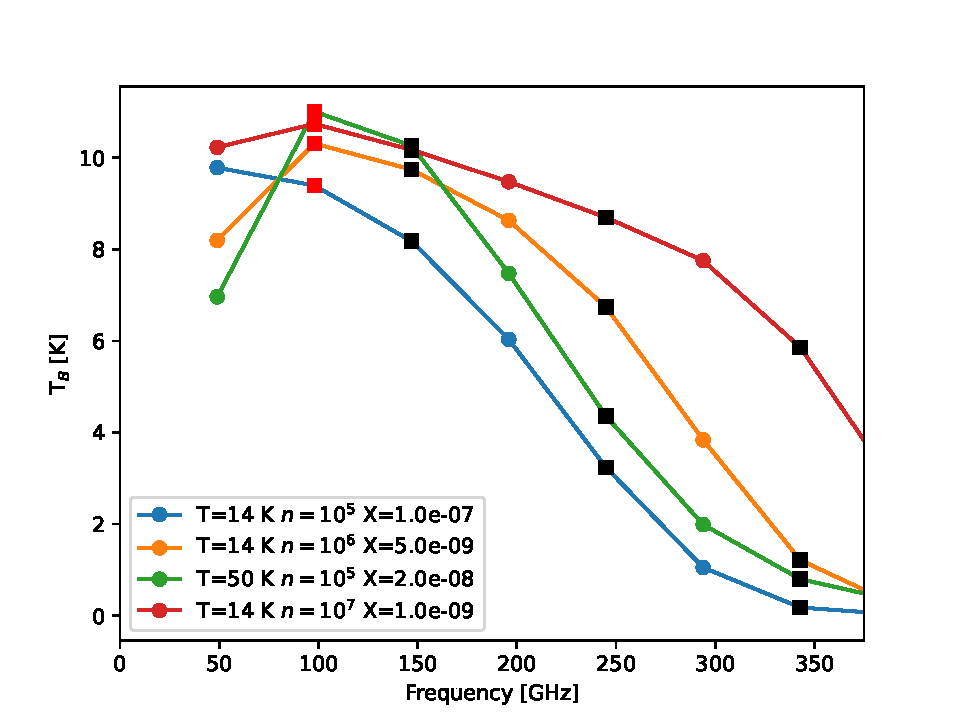
\includegraphics[width=0.55\textwidth]{figures/proposal_figures/CS_RADEX_models_withobs.pdf}
    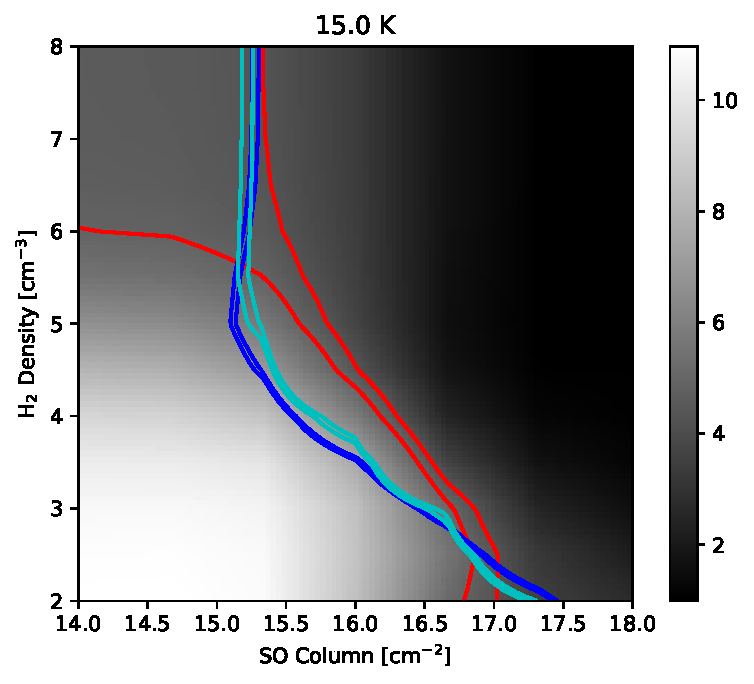
\includegraphics[width=0.42\textwidth]{figures/RADEX_SOratio_model_T=15.0.pdf}
    \caption{(left) Model CS spectral line energy distribution showing the necessity of multi-frequency coverage to distinguish between different excitation models.
    Only one line, CS 2-1 at 98 GHz, has been observed (red squares), and it is compatible with a range of densities and temperatures.
    To distinguish high temperature from high density, accounting for different possible abundances, we need to observe a wide range of frequencies (black squares).
    This model is tuned for the proposed observations (which have sensitivity 0.25 - 2 K) assuming the filling factor was $\sim0.1$ in the archival 2" resolution data.
    The true brightness could be as much as $10\times$ greater.
    (right) RADEX non-LTE model for SO extracted from \citet{Ginsburg2024}.
    The contours show the regions of parameter space allowed by the archival observations, and the colorscale shows the 2(3)-1(2) to 2(2)-1(1) ratio.
    SO's rotational levels are split by spin-rotation coupling such that there are often several transitions with similar observed frequency but significantly different energy levels in a given ALMA band.
    This feature makes SO a particularly powerful tool for measuring gas excitation conditions \citep{Lique2007}.
    }
    \label{fig:csradex}
\end{figure}

% \begin{figure}
%     \centering
%     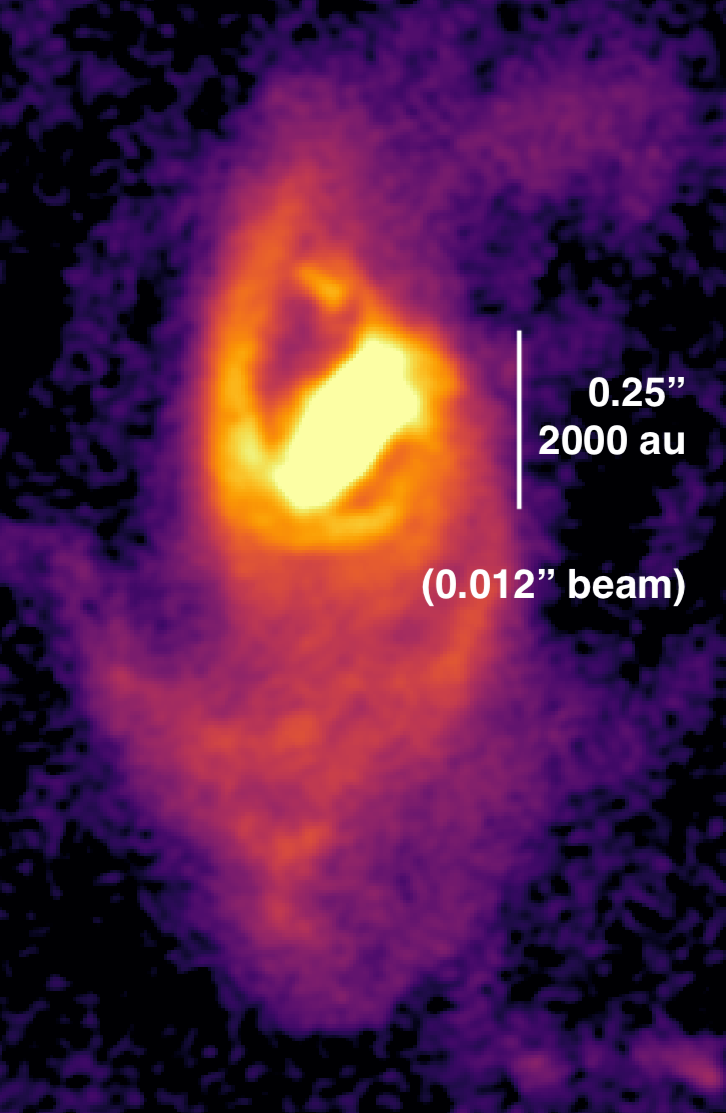
\includegraphics[width=0.35\textwidth]{figures/proposal_figures/sgrc_disk_zoom_scalebar.png}
%     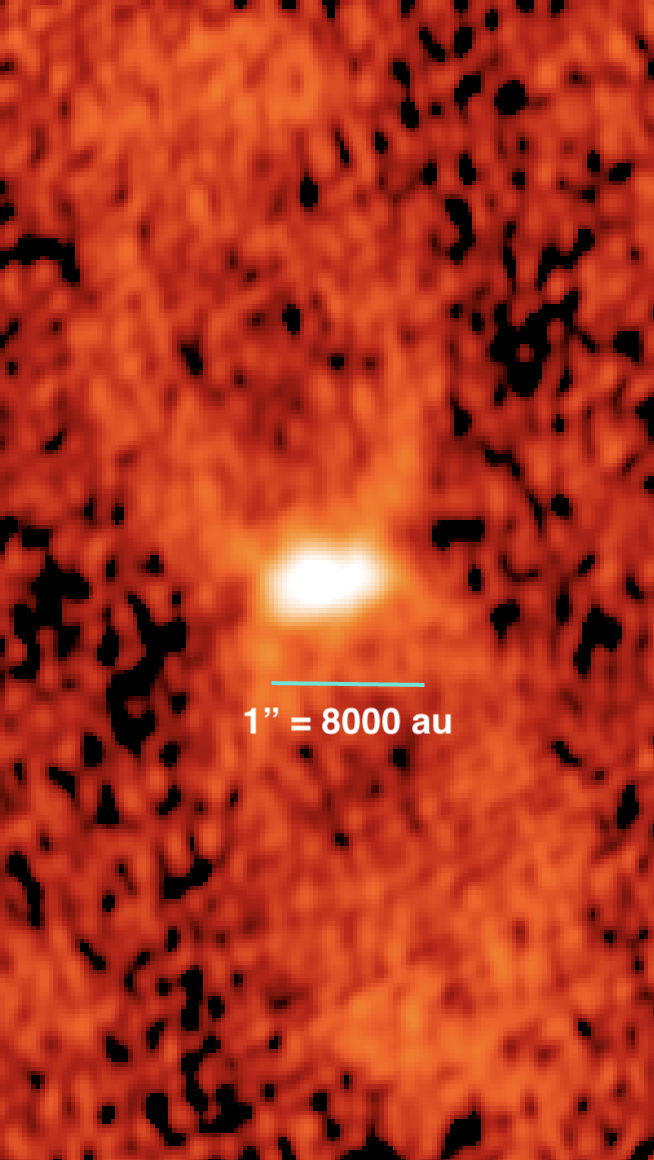
\includegraphics[width=0.30\textwidth]{figures/proposal_figures/CKVulcontinuum.png}
%     \caption{Example images of what we might detect in the proposed observations.
%     Left shows a large ($\sim2000$ au), massive (5 \msun) disk \citep{Lu2022} observed in the Galactic Center with ALMA at B7 in C10 in 2023.
%     Right shows CK Vulpecula \citep{Eyres2018} observed with ALMA in B6, the remnant of a white dwarf-brown dwarf merger that bears a different kind of disk, scaled to the distance of the Galactic Center.  
%     The central source in each of these objects has a similar continuum flux (to within a factor of a few) to the MUBLO in the 2" beam that is presently the only detection of the MUBLO.
%     }
%     \label{fig:whatwecouldsee}
% \end{figure}
% CK Vul image member.uid___A001_X129e_X258.CK_Vul_sci.spw25_27_29_31.cont.I.pbcor.fits

%\section{References}

% List references here
% Minimum font size for references: 12pt 
% Proposals not compliant to this will be rejected. See Section 5.3.1 in the ALMA Proposer's Guide.

\bibliography{main}{}
\bibliographystyle{aasjournal}


%%%%%%%%%%%%%%%%%%%%%%%%%%%
%%%%% End of document %%%%%
%%%%%%%%%%%%%%%%%%%%%%%%%%%

\end{document}

